% Exercise Template
% A LaTeX template for typesetting exercise in Persian (with cover page).
% By: Reza Adinepour
% Github: github.com/rezaAdinepour

\documentclass[12pt]{exam}

\usepackage{setspace}
\usepackage{listings}
\usepackage{graphicx,wrapfig}
\usepackage{caption}
\usepackage{subcaption}
\usepackage{multirow}
\usepackage{matlab-prettifier}
\usepackage{amsmath}
\usepackage{multicol}
\usepackage[hidelinks]{hyperref}



\usepackage[utf8]{inputenc}
\usepackage{fourier} 
\usepackage{array}
\usepackage{makecell}

\renewcommand\theadalign{bc}
\renewcommand\theadfont{\normalsize}
\renewcommand\theadgape{\Gape[4pt]}
\renewcommand\cellgape{\Gape[4pt]}


\usepackage[margin=25mm]{geometry}
\usepackage{xepersian}
\settextfont{XB Niloofar}

\newcommand{\class}{\ThesisClass}

\singlespacing
\parindent 0ex

\begin{document}


% -------------------------------------------------------
%  Thesis Information
% -------------------------------------------------------

\newcommand{\ThesisType}
{سمینار}  % پایان‌نامه / رساله
\newcommand{\ThesisDegree}
{کارشناسی ارشد گرایش معماری کامپیوتر}  % کارشناسی / کارشناسی ارشد / دکتری
\newcommand{\ThesisMajor}
{مهندسی کامپیوتر}  % مهندسی کامپیوتر
\newcommand{\ThesisTitle}
{تمرین شبیه‌سازی اول}
\newcommand{\ThesisAuthor}
{نام دانشجو\\شماره دانشجویی}
\newcommand{\ThesisClass}
{درس فناوری های حافظه\\دکتر حامد فربه}
\newcommand{\ThesisSemester}
{CE5431 | بهار ۱۴۰۳}
\newcommand{\ThesisDate}
{اسفند 1402}
\newcommand{\ThesisDepartment}
{دانشکده مهندسی کامپیوتر}


\newcommand{\ThesisGroupNameI}
{مرتضی عادلخانی (\href{mailti:madelkhani@aut.ac.ir}{\textcolor{blue}{madelkhani@aut.ac.ir}})}
\newcommand{\ThesisGroupNameII}
{سارا زمانی (\href{mailti:sara.zamani73@aut.ac.ir}{\textcolor{blue}{sara.zamani73@aut.ac.ir}})}


\newcommand{\ThesisUniversity}
{دانشگاه صنعتی امیرکبیر}

% -------------------------------------------------------
%  English Information
% -------------------------------------------------------

\newcommand{\EnglishThesisTitle}{A Standard Template for Course Exercise}


\pagestyle{empty}

\begin{center}

\includegraphics[scale=0.18]{images/aut-fa2.png}

%\vspace{0.5cm}
%\ThesisUniversity \\[-0.3em]
%\vspace{0.5cm}
\large\ThesisDepartment

\begin{large}
\vspace{0.5cm}


%\ThesisMajor

\end{large}

\vspace{1cm}


{\large\textbf{\ThesisClass}}
\vspace{1cm}

%{نگارش}\\[.5em]
{\large\textbf{\ThesisAuthor}}


\vspace{1.5cm}

{\LARGE\textbf{\ThesisTitle}}\\ 
\vspace{2cm}





% \begin{latin}
% {\Large\textbf\EnglishThesisTitle}
% \end{latin}

{تدریسیار:}\\[.8em]

\ThesisGroupNameI \\
\ThesisGroupNameII



\vspace{3cm}



\ThesisSemester

\end{center}

\newpage


% These commands set up the running header on the top of the exam pages
\pagestyle{head}
\firstpageheader{}{}{}
\runningheader{صفحه \thepage\ از \numpages}{}{\class}
\runningheadrule

\newcommand{\tf}[1][{}]{%
	\fillin[#1][0.25in]%
}


\vspace{0pt}


\begin{questions}
	\pointpoints{نمره}{نمره}



	\section{سوالات صحیح و غلط}
	
	
	%%%%%%%%%%%%%%%%%%%%%%%%%%%%%%% T/F Q1 %%%%%%%%%%%%%%%%%%%%%%%%%%%%%%%
	\printanswers
	\question
	\lr{PCM}\footnote{\lr{Phase change memory}} ها نسبت به \lr{DRAM} ها از نظر فناوری مقیاس‌پذیری بیشتری دارند.
	 
	 \begin{checkboxes}
	 	\CorrectChoice درست
	 	 \choice غلط
	 \end{checkboxes}
	 
	 \textbf{توضیح:} در \lr{DRAM} ها به دلیل وجود خازن، اندازه ترانزیستور‌ها و خازن را نمی‌توان از حدی کوچک‌تر کرد اما در \lr{PCM} ها به دلیل به دلیل استفاده از موادی که تغییر فاز ایجاد می‌کنند می‌توان حافظه‌های چگال تری به نسبت \lr{DRAM} ها ساخت	 
	
	
	
	%%%%%%%%%%%%%%%%%%%%%%%%%%%%%%% T/F Q2 %%%%%%%%%%%%%%%%%%%%%%%%%%%%%%%
	\printanswers
	\question
	عملیات خواندن و نوشتن در \lr{PCM} ها به نسبت \lr{DRAM} ها، بازده انرژی بیشتری دارد.
	
	 \begin{checkboxes}
		\choice درست
		\CorrectChoice غلط
	\end{checkboxes}
	
	\textbf{توضیح:} فرایند نوشتن در \lr{DRAM} شامل یک تخلیه بار خازن است که انرژی زیادی را متحمل نمی‌شود. اما همین عملیات نوشتن در \lr{PCM} نیازمند انرژی بالایی‌ست 
	
	
	%%%%%%%%%%%%%%%%%%%%%%%%%%%%%%% T/F Q3 %%%%%%%%%%%%%%%%%%%%%%%%%%%%%%%
	\printanswers
	\question
	\lr{PCM} تاخیر دسترسی کمی دارد اما در مقایسه با حافظه \lr{Nand Flash}، استقامت\footnote{\lr{Endurance}} دراد. 
	
	\begin{checkboxes}
		\choice درست
		\CorrectChoice غلط
	\end{checkboxes}
	
	\textbf{توضیح:} \lr{PCM} ها به دلیل توانایی سریع تعویض حالت، سرعت خواندن و نوشتن بالایی را ارائه می‌دهند که منجر به تاخیر دسترسی کمتری می‌شود. اما نسبت به \lr{Nand Flash} تعداد کمتری می‌تواند در آن نوشته و از آن خوانده شود قبل از آنکه خراب شود
	
	
	%%%%%%%%%%%%%%%%%%%%%%%%%%%%%%% T/F Q4 %%%%%%%%%%%%%%%%%%%%%%%%%%%%%%%
	\printanswers
	\question
	\lr{NVM} استقامت کمتری نسبت به \lr{DRAM} دارد. زیرا فرایند نوشتن در \lr{NVM} بسیار بیشتر طول می‌کشد.
	
	\begin{checkboxes}
		\choice درست
		\CorrectChoice غلط
	\end{checkboxes}
	
	\textbf{توضیح:} حافظه‌های غیر فرار، استقامت کمتری نسبت به \lr{DRAM} ها دارند اما دلیل استقامت کم در صورت سوال به اشتباه بیان شده است. به دلیل مکانیزم پیچیده‌تر نسبت به \lr{DRAM} ها استقامت کمتری دارند.
	
	
	
	
	
	
	
	
	
	
	
	
	
	
	\section{سوالات چند گزینه‌ای}
	%%%%%%%%%%%%%%%%%%%%%%%%%%%%%%% M/C Q1 %%%%%%%%%%%%%%%%%%%%%%%%%%%%%%%
	\printanswers
	\question
	کدام یک از گزینه‌های زیر یکی از اشکالات استفاده از حافظه \lr{Nand Flash} به‌عنوان فایل سیستم را مطرح می‌کند؟
	
	\begin{checkboxes}
		\choice داده‌های ذخیره شده در آن با گذشت زمان از بین می‌روند و نیاز به بازتجدید دارند
		\choice سرعت خواندن از آن غیرقابل پیش‌بینی است و چالش‌هایی را برای زمان‌بندی \lr{I/O} ایجاد می‌کند
		\item زمان جستجو به طور قابل توجهی در مقایسه با دیسک های سنتی طولانی تر است
		\CorrectChoice به دلیل پشتیبانی محدود، محدودیت هایی را بر تعداد نوشتن در هر بلوک اعمال می کند.
	\end{checkboxes}
	
	\textbf{توضیح:} حافظه \lr{Nand flash} به حافظه ای با تعداد محدود نوشتن و پاک کردن \lr{Program/Erase} معروف است به همین دلیل این گزینه صحیح است.
	
	
	







	
	
	
	\section{سوالات جای خالی}
	%%%%%%%%%%%%%%%%%%%%%%%%%%%%%%% Fill Q1 %%%%%%%%%%%%%%%%%%%%%%%%%%%%%%%
	\question
	جدول زیر را با بهترین جمله تکمیل کنید.
	
	\begin{latin}
		\begin{center}
			\resizebox{\columnwidth}{!}{%
			\begin{tabular}{||c c c c c c||} 
				\hline
				& \textbf{Registers} & \textbf{SRAM} & \textbf{DRAM} & \thead{\textbf{HARD} \\ \textbf{Disk}} & \textbf{Flash} \\ [0.5ex] 
				\hline\hline
				\textbf{Approx. Access Time (ns or s)} & $\approx1 ns$ & $\approx2-10 ns$ & $\approx10-100 ns$ & $\approx5-10ms$ & $\approx25-50\mu s$ \\ 
				\hline
				\textbf{Density (Mb/area)} & Very low & Low & High & Very high & High\\
				\hline
				\textbf{Volatility} & Volatile & Volatile & Volatile & Non-volatile & Non-volatile\\
				\hline
				\textbf{Approx. Cost/Bit (\$)} & Very High & High & Medium & Very low & Low\\
				\hline
				\textbf{Power Usage (W)} & High & Medium & Low & Medium & Low\\
				\hline
				\textbf{Composition} & Flip-flops & Transistors & Capacitors & Magnetic storage & Floating gate transistors \\ 
				\hline
				\textbf{Example Usage} & FPGAs & L2\&L3 cache & Main memory & Hard disk & MicroSD \\ [1ex] 
				\hline
			\end{tabular}
		}
		\end{center} 
	\end{latin}
	
	
	
	
	
	
	
	
	
	
	
	
	
	
	
	
	
	
	\section{سوالات تعریفی}
	%%%%%%%%%%%%%%%%%%%%%%%%%%%%%%% Diff Q1 %%%%%%%%%%%%%%%%%%%%%%%%%%%%%%%
	\question
	\textbf{یک سلول \lr{SRAM-6T} را درنظر بگیرید که برای پایداری در شرایط کاری بهینه شده است. به سوالات زیر پاسخ دهید.}
	
	
	\begin{enumerate}
		\item \textbf{افزایش ولتاژ \lr{Wordline} چه تاثیری بر پایداری خواندن سلول دارد؟}
		افزایش ولتاژ \lr{Wordline} باعث کاهش پایداری خواندن می‌شود زیرا باعث افزایش قدرت \lr{access} ترانزیستور شده و در نتیجه احتمال خراب شدن سلول حافظه را افزایش می‌دهد.
		
		
		\textbf{\item افزایش ولتاژ \lr{Wordline} چه تاثیری بر زمان دسترسی خواندن دارد؟}
افزایش ولتاژ \lr{Wordline} زمان دسترسی خواندن را کاهش می‌دهد زیرا باعث افزایش قدرت هدایت N0 می‌شود.
		
		
		\textbf{\item افزایش ولتاژ \lr{Wordline} چه تاثیری بر قابلیت نوشتن در سلول دارد؟}
افزایش ولتاژ \lr{Wordline} قابلیت نوشتن در سلول را بهبود می بخشد زیرا \lr{Access} ترانزیستور با قدرت بیشتری هدایت می‌کند و در نتیجه احتمال غلبه بر سلول SRAM افزایش می یابد.
		
		\textbf{\item یک پالس \lr{Wordline} کوتاه شده چگونه بر ثبات خواندن سلول تاثیر می‌گذارد؟}
کاهش زمان پالس \lr{Wordline} پایداری خواندن را بهبود می بخشد زیرا کل جریان کشیده شده از سلول SRAM را کاهش می دهد.
		
		\textbf{\item طولانی شدن \lr{Wordline} چه تاثیری بر خوانایی سلول دارد؟}
افزایش طول پالس \lr{Wordline} قابلیت نوشتن در سلول را بهبود می بخشد زیرا به \lr{Access} ترانزیستور زمان بیشتری برای خواندن می‌دهد.
		
		\textbf{\item افزایش ولتاژ منبع تغذیه چگونه بر قابلیت نوشتن سلول تاثیر می‌گذارد؟}
افزایش ولتاژ تغذیه سلول SRAM باعث کاهش قابلیت نوشتن آن می‌شود. افزایش \lr{VDD} توانایی سلول \lr{SRAM} را برای حفظ داده‌ها افزایش می‌دهد، بنابراین نوشتن در سلول را سخت‌تر می‌کند.
	\end{enumerate}
	
	
	
	
	
	
	\question
\textbf{حافظه دسترسی تصادفی مقاومتی مغناطیسی (\lr{MRAM}) و حافظه تغییر فاز (\lr{PRAM} یا \lr{PCRAM}) نشان دهنده دو نوع حافظه غیر فرار با کاربردهای بالقوه در دستگاه های مصرف کننده آینده و سیستم های تعبیه شده است. این فناوری‌ها را با توضیح اصول عملیاتی، مزایای اصلی به عنوان جایگزینی برای \lr{DRAM} و یا \lr{SRAM}، مزایای طراحان سیستم‌های جاسازی شده، محدودیت‌ها و زمینه‌هایی که ممکن است مناسب نباشند، مقایسه و مقایسه کنید.}


\lr{MRAM} داده‌ها را با استفاده از حالت‌های مغناطیسی ذخیره می‌کند. این حافظه شامل پیوندهای تونلی مغناطیسی (\lr{MTJ}) است که داده‌ها را با تغییر جهت‌گیری لایه‌های مغناطیسی درون پیوند می‌نویسد. خواندن داده‌ها شامل اندازه‌گیری مقاومت \lr{MTJ} است که بر اساس جهت‌گیری نسبی لایه‌های مغناطیسی (موازی یا ضد موازی) متفاوت است.


\lr{PRAM} داده‌ها را با تغییر فاز یک ماده چالکوژنید (معمولاً ترکیبی مانند \lr{Ge2Sb2Te5}) ذخیره می‌کند. با اعمال گرما از طریق پالس‌های الکتریکی، بین حالت آمورف (مقاومت بالا) و حالت بلوری (مقاومت پایین) تغییر فاز می‌دهد.

از مزایای اصلی \lr{MRAM} می‌توان به:
\begin{enumerate}
	\item زمان خواندن و نوشتن سریع، قابل مقایسه با \lr{SRAM}.
	\item دوام بالای نوشتن، قادر به تحمل تعداد زیادی چرخه نوشتن.
	\item غیر فرار بودن
	\item در مقایسه با \lr{DRAM } مصرف انرژی کمی دارد زیرا مانند \lr{DRAM} ها نیازی به آپدیت داده ندارد.
\end{enumerate}

اشاره کرد. همچنین از مزایای \lr{PRAM} نیز می‌توان موارد زیر را نام برد:
\begin{enumerate}
	\item چگالی ذخیره‌سازی بالاتر نسبت به \lr{}، نزدیک به حافظه فلش \lr{NAND}.
	\item غیر فرار بودن
	\item قابلیت مقیاس‌پذیری بالا به دلیل ساختار ساده و استفاده از موادی که می‌توانند به ابعاد کوچکتر مقیاس شوند.
	\item سرعت خواندن سریع‌تر نسبت به حافظه فلش \lr{NAND} سنتی.
\end{enumerate}

از محدودیت‌های این دو حافظه می‌توان به موارد زیر اشاره نمود:
\begin{enumerate}
	\item در حال حاضر هزینه تولید \lr{MRAM} آن نسبت به سایر حافظه‌های غیر فرار مانند فلش \lr{NAND} گران‌تر است.
	
	\item 
	\lr{MRAM} چگالی ذخیره‌سازی پایین‌تری نسبت به \lr{PRAM} و فلش \lr{NAND} دارد.
	
	\item 
سرعت نوشتن در \lr{PRAM} عموماً کندتر از \lr{MRAM} و \lr{DRAM}، که ممکن است برای برخی کاربردهای با سرعت بالا محدودیت ایجاد کند.
\end{enumerate}

بنابر این می‌توان گفت هر دو حافظه \lr{MRAM} و \lr{PRAM} مزایای قابل توجهی برای دستگاه‌های مصرفی آینده و سیستم‌های نهفته دارند. \lr{MRAM} در سرعت و دوام برتری دارد و PRAM چگالی بالاتر و مقیاس‌پذیری بهتری ارائه می‌دهد. انتخاب بین آن‌ها بستگی به نیازهای خاص کاربرد، از جمله سرعت، دوام، چگالی و ملاحظات مصرف انرژی دارد.





\question
\textbf{نقش فناوری \lr{SSD} را در تغییر مسیر از هارد دیسک (\lr{HDD}) به سمت ذخیره سازی حالت جامد، به ویژه در حوزه لوازم الکترونیکی مصرفی و زیرساخت های سازمانی، تجزیه و تحلیل کنید.}

تغییر از \lr{HDD}‌ها به \lr{SSD}‌ها در هر دو حوزه الکترونیک مصرفی و زیرساخت‌های سازمانی به دلیل عملکرد برتر، دوام، بهره‌وری انرژی و مزایای اندازه، سرعت بالا صورت گرفته است. دسترسی سریع‌تر به داده‌ها، مقیاس‌پذیری بهتر و کاهش هزینه‌های عملیاتی را امکان‌پذیر کرده‌اند. با پیشرفت فناوری و کاهش قیمت‌ها، \lr{SSD}‌ها به احتمال زیاد به راه‌حل ذخیره‌سازی اصلی تبدیل می‌شوند و کاهش استفاده از \lr{HDD}‌ها در اکثر کاربردها را تسریع می‌کنند. اما همچنان به دلیل وجود بازار برای \lr{HDD} ها این فناوری هنوز از رده خارج نشده است و مورد استفاده قرار می‌گیرد.





\question
\textbf{پروتکل رابط \lr{NVMe} و برتری آن را نسبت به رابط های معمولی مرتبط با \lr{HDD} مانند \lr{SATA}، با تاکید بر معیارهای عملکرد مانند نرخ انتقال، توضیح دهید.}


رابط پروتکل \lr{NVMe} به طور قابل توجهی برتر از رابط‌های سنتی مانند \lr{SATA} است، به ویژه از نظر نرخ انتقال داده و تأخیر. \lr{NVMe} با استفاده از پهنای باند بالا و قابلیت‌های چند مسیره \lr{PCIe}، سرعت‌های خواندن و نوشتن بسیار بالاتر و تأخیر کمتری را ارائه می‌دهد. این مزایا، همراه با بهینه‌سازی‌های بهره‌وری \lr{CPU} و کاهش مصرف انرژی، \lr{NVMe} را به انتخاب اصلی برای حافظه‌های غیر فرار مدرن تبدیل کرده است، که نیازهای عملکردی بالای سیستم‌های امروزی را برآورده می‌کند.






\question
\textbf{بین یک ترانزیستور  فلوتینگ گیت و یک ماسفت مسطح استاندارد از نظر ترکیب ساختاری آنها تفاوت قائل شوید. اهمیت عدم اتصال مستقیم دروازه شناور به پایانه های خارجی را توضیح دهید.}


ترانزیستور فلوتینگ گیت و ماسفت استاندارد دارای تفاوت‌های ساختاری عمده‌ای هستند که به کاربردهای مختلف آنها منجر می‌شود. عدم اتصال مستقیم گیت شناور به ترمینال‌های خارجی، قابلیت‌های ذخیره‌سازی غیر فرار و حفظ داده‌ها را به ترانزیستور فلوتینگ گیت می‌دهد، که آن را برای حافظه‌های فلش و دیگر کاربردهای حافظه‌های غیر فرار مناسب می‌سازد.















\section{سوالات سناریوای}
%%%%%%%%%%%%%%%%%%%%%%%%%%%%%%% Scenario %%%%%%%%%%%%%%%%%%%%%%%%%%%%%%%
\question
\textbf{توسعه یک سیستم کامپیوتری برای یک ماموریت فضای عمیق گسترده با هدف کاوش در یک سیاره فراخورشیدی از راه دور به شما اختصاص داده شده است. این ماموریت شامل کسب و تجزیه و تحلیل داده های علمی قابل توجه در یک دوره طولانی، با پهنای باند محدود برای انتقال داده ها به زمین خواهد بود. این فضاپیما به انواع حسگرها، دوربین ها و دستگاه های علمی برای جمع آوری اطلاعات در مورد شرایط جوی سیاره فراخورشیدی، ویژگی های زمین شناسی و نشانه های احتمالی حیات مجهز خواهد شد.}


\textbf{چالش اول: }\\
\textbf{یک معماری برای سیستم کامپیوتری ابداع کنید که از یک سلسله مراتب حافظه ساختاریافته استفاده می کند، که انواع مختلف حافظه غیر فرار را در خود جای می دهد تا داده های به دست آمده در طول ماموریت فضای عمیق را مدیریت کند. واحد حافظه بهینه را برای هر ردیف از سلسله مراتب با در نظر گرفتن عوامل زیر انتخاب کنید:}

\begin{enumerate}
	\item
\textbf{	نیاز به خاطرات غیرفرار قابل اعتماد و سخت شده در فضا که می توانند در محیط شدید فضایی مقاومت کنند.}
	
	\item 
\textbf{	رویکردهایی برای کاهش مصرف انرژی و افزایش ظرفیت ذخیره سازی، با توجه به محدودیت های قدرت و اندازه فضاپیما.}
	
	\item 
\textbf{	تکنیک هایی برای حفظ یکپارچگی داده ها و کاهش احتمال از دست دادن داده ها یا خراب شدن در طول مدت ماموریت}
	
	\item 
\textbf{ادغام ویژگی‌های تحمل‌پذیر خطا برای رسیدگی به نقص‌های احتمالی سخت‌افزار یا خطاهای ناشی از تشعشع}
	
	\item 
\textbf{	روش‌هایی برای دسترسی و پردازش مؤثر داده‌ها، با در نظر گرفتن قابلیت‌های محاسباتی محدود فضاپیما}
	
	\item 
\textbf{	هماهنگ سازی سیستم های حافظه غیر فرار با سایر عناصر سیستم کامپیوتری مانند \lr{CPU} ها، رابط های ارتباطی و واحدهای کنترل قدرت.}
\end{enumerate}


\textbf{چالش دوم:}\\
\textbf{برای هر بخش از سلسله مراتب حافظه (به عنوان مثال، حافظه پنهان، حافظه اولیه، حافظه ثانویه)، مناسب ترین نوع حافظه غیر فرار (به عنوان مثال، \lr{NAND flash}، \lr{NOR flash}، حافظه تغییر فاز، حافظه با دسترسی تصادفی مقاومتی) را شناسایی کنید. در مورد ویژگی های آن و خواسته های منحصر به فرد ماموریت. با توضیح اینکه چگونه هر نوع حافظه با جنبه های حیاتی فوق الذکر مطابقت دارد، از انتخاب های خود حمایت کنید.}


\textbf{چالش سوم:}\\
\textbf{پیشنهاد یک استراتژی احتمالی و تکراری برای زیرسیستم حافظه غیر فرار برای تضمین حفاظت از داده های ضروری در صورت بروز نقص شدید یا بی نظمی پیش بینی نشده در طول ماموریت. مناسب ترین روش افزونگی (به عنوان مثال، تکرار، برابری، \lr{RAID}) و پروتکل پشتیبان (به عنوان مثال، تکرار منظم داده ها در یک واحد ذخیره سازی پشتیبان، کدهای تصحیح خطا) را برای هر سطح سلسله مراتب حافظه تعیین کنید. توضیح دهید که چگونه استراتژی شما خطرات را به حداقل می رساند و به موفقیت ماموریت کمک می کند.}


\textbf{پاسخ:}\\
برای طراحی این حافظه جنبه‌های مختلفی را باید بررسی کنیم. از آنجایی که قرار است این حافظه در محیطی غیر معمول مورد استفاده گیرد ابتدا می‌بایست چالش‌های طراحی را پیدا کنیم. برای این مسئله چالش‌های زیر مطرح است:

\begin{enumerate}
	\item محیط فضا دماهای بسیار بالا (یا بسیار پایین) و سطوح بالای تابش را ارائه می‌دهد که می‌تواند به قطعات الکترونیکی معمولی آسیب برساند.
	
	برای حل این مشکل می‌توان از فناوری های حافظه ای استفاده نمود که به‌طور خاص برای مقاومت در برابر چنین شرایط جوی ای طراحی شده است. این حافظه‌ها شامل نسخه‌های خاص از \lr{NAND Flash} و \lr{NOR} \lr{Flash}، و همچنین فناوری‌های جدیدتری مانند حافظه \lr{PCM} و \lr{RAM} مقاومتی (\lr{ReRAM}) که به طور ذاتی در برابر تابش مقاوم‌تر هستند.
	
	\item 
	مشکل دوم مسئله محدودیت‌های برقی و توانی در فضاپیماست.
	
	پیاده‌سازی یک سلسله‌مراتب حافظه که در هر سطح تعادل بین مصرف برق، ظرفیت و عملکرد را حفظ کند. با استفاده از فناوری‌های حافظه کم‌مصرف و اعمال تکنیک‌هایی مانند فشرده‌سازی داده و مدیریت کارآمد برق می‌توان این چالش را حل نمود
	
	\item 
	مشکل بعد، اطمینان از اینکه داده‌ها در طول مدت طولانی دقیق و بدون خطا باقی می‌مانند.
	
	برای حل این مشکل استفاده از کدهای تصحیح خطا (\lr{ECC}) و پیکربندی‌های \lr{RAID} برای تشخیص و تصحیح خطاها استفاده نمود.
	
	\item 
	خرابی‌های سخت‌افزاری و خطاهای ناشی از تابش.
	
	برای حل این مشکل، می‌توان با گنجاندن افزونگی و اصول طراحی مقاوم در برابر خطا مانند سیستم‌های حافظه دوگانه افزونه، تایمرهای نگهبان، و پروتکل‌های بازیابی خطا استفاده نمود.
	
	\item 
	مشکل بعدی قابلیت‌های محاسباتی محدود در فضاپیماست. برای حل این مشکل می‌بایست از الگوریتم های پردازشی \lr{Quantized} شده استفاده نمود تا با کمترین تغییر دقت حافظه کمتری مصرف کنیم.
\end{enumerate}



در چالش  دوم، سلسله مراتب حافظه را به‌صورت زیر پیشنهاد می‌دهم:

\begin{enumerate}
	\item استفاده از \lr{SRAM} در کش. زیرا \lr{SRAM} سریع است و برای حافظه کش مناسب است به دلیل تأخیر کم آن. اگرچه فرار است، اما استفاده از نسخه‌های مقاوم در برابر تابش می‌تواند قابلیت اطمینان را حفظ کند.
	
	\item 
	استفاده از \lr{PCM} و \lr{MRAM} برای حافظه اصلی. زیرا این دو حافظه  غیر فرار هستند، زمان دسترسی سریعی دارند همچنین مقاومت خوبی نیز دارند. \lr{PCM} به ویژه در برابر تابش و دماهای بالا مقاوم است.
	
	\item 
	در حافظه ثانویه می‌توان از \lr{Nans flash} استفاده کرد. زیرا  ظرفیت ذخیره‌سازی بالایی را فراهم می‌کند و همچنین غیر فرار است. نسخه‌های مقاوم در برابر تابش آن نیز موجود است.
	
	\item 
	در حافظه بلند‌مدت می‌توان از \lr{ReRAM} ها استفاده کرد. زیرا بسیار مقاوم است، مصرف برق کمی دارد و می‌تواند داده‌ها را برای مدت طولانی نگه دارد، که آن را برای ذخیره‌سازی بلندمدت در محیط‌های سخت مناسب کرده است.
\end{enumerate}


برای حل چالش سوم و در هر سطح حافظه پیشنهادات زیر را ارائه می‌دهم.

\begin{enumerate}
	\item در کش ها می‌توان از روش \lr{DMR} برای بررسی خطا به صورت \lr{Real-time} استفاده نمود
	
	\item 
	 در حافظه اصلی نیز می‌توان برای بررسی و تصحیح خطاها از \lr{DMR} استفاده نمود. زیرا در اینجا نیز پیدا و تصحیح خطاها باید به صورت \lr{Real time} انجام شود.
	 
	 \item 
	 در حافظه ثانویه می‌توان از \lr{RAID} استفاده نمود. \lr{RAID} تحمل خطا را با توانایی بازیابی از دو خرابی دیسک همزمان فراهم می‌کند. تکثیر منظم داده‌ها اطمینان می‌دهد که همیشه یک نسخه ثانویه در دسترس است.
	 
	 \item 
	 در حافظه بلندمدت می‌نوان حافظه را به‌صورت دوره ای بررسی نمود.
\end{enumerate}















\section{سوالات طراحی}
%%%%%%%%%%%%%%%%%%%%%%%%%%%%%%% Design %%%%%%%%%%%%%%%%%%%%%%%%%%%%%%%
\question
\textbf{هدف شما در این کار ایجاد مدار برای یک \lr{ROM} دو پورت است که 4 بیت عرض و 4 کلمه عمق دارد. این \lr{ROM} دارای دو پورت مجزا است که هر کدام مجهز به یک گذرگاه آدرس 2 بیتی و یک گذرگاه داده 4 بیتی است که امکان دسترسی همزمان به هر یک از چهار کلمه داده ذخیره شده را فراهم می کند. فرآیند طراحی را با تطبیق سلول های ROM تک پورت اولیه ارائه شده آغاز کنید. پس از آن، یک طرح شماتیک مدار برای کل ROM دو پورت، که شامل تمام مدارهای ضروری است، ترسیم کنید. محتویات رام در زیر به تفصیل آمده است.}


\begin{figure}[h]
	\centering
	\includegraphics[width=0.9\textwidth]{images/img1}
\end{figure}

مدار طراحی پیشنهادی به صورت زیر است:


در این طراحی، هر بلوک آدرس نشان دهنده سلول های ROM است که کلمات 4 بیتی را ذخیره می کند. دیکدر آدرس، کلمه مناسب را بر اساس آدرس ورودی انتخاب می کنند، و مالتی پلکسرها اطمینان حاصل می‌شود که داده های صحیح به گذرگاه های داده خروجی برای هر پورت هدایت می شود یا خیر


\begin{figure}[h]
	\centering
	\includegraphics[width=0.7\textwidth]{images/img2/img2.pdf}
\end{figure}













	
%\textbf{	یک شرکت فناوری در حال توسعه یک شتاب دهنده شبکه عصبی با معماری پردازش در حافظه (\lr{PIM}) برای استفاده در سیستم های اتوماسیون صنعتی است. معماری \lr{PIM} اجازه می دهد تا محاسبات به طور مستقیم در دستگاه های حافظه انجام شود، حرکت داده ها را کاهش می دهد و کارایی انرژی را بهبود می بخشد. این شرکت برای پیاده سازی ساختار PIM در شتاب دهنده شبکه عصبی باید بین دستگاه های حافظه مختلف مانند SRAM، DRAM، MRAM و PCM تصمیم بگیرد.}
%	
%\textbf{	در زمینه شتاب دهنده شبکه عصبی صنعتی ما با ساختار پردازش در حافظه (\lr{PIM})، مناسب بودن دستگاه های حافظه مختلف (\lr{SRAM}، \lr{DRAM}، \lr{MRAM}، \lr{PCM}) را برای اجرای \lr{PIM} مقایسه کنید. عواملی مانند سرعت دسترسی، بهره وری انرژی، استقامت، کارایی منطقه و سهولت یکپارچه سازی را در نظر بگیرید. ارائه یک توصیه بر اساس الزامات و محدودیت های خاص برنامه اتوماسیون صنعتی.}
%	
%\textbf{بر اساس تجزیه و تحلیل، مناسب ترین دستگاه حافظه (\lr{SRAM}، \lr{DRAM}، \lr{MRAM}، \lr{PCM}) را برای پیاده سازی ساختار پردازش در حافظه (\lr{PIM}) در شتاب دهنده شبکه عصبی برای اتوماسیون صنعتی توصیه کنید. توصیه خود را با همسویی با الزامات خاص، اهداف عملکرد و محدودیت‌های برنامه اتوماسیون صنعتی توجیه کنید. در مورد مبادلات بالقوه و هرگونه ملاحظات اضافی که بر تصمیم شما تأثیر گذاشته است بحث کنید.}
%	
%	
%	
%برای این‌که بتوان یکی از ساختار‌های حافظه بیان شده را انتخاب کرد، نیاز است که اپلیکیشن به طور کامل بر ما روشن باشد اما با توجه به این‌که در این سوال اپلیکیشن برای ما به طور واضح مشخص نیست، ویژگی‌های حافظه‌های مظرح شده را بیان می‌کنیم و درنهایت بر‌اساس ویژگی‌های بیان شده و یک اپلیکیشن فرضی یک یا چند حافظه را پیشنهاد می‌دهیم.
%
%عوامل کلیدی و مهم برای انتخاب یک حافظه به عنوان \lr{PIM} برای پردازش شبکه‌های عصبی، شامل سرعت دسترسی\footnote{\lr{Access time}}، انرژی، استقامت\footnote{Endurance}، مساحت مصرفی، مقیاس‌پذیری\footnote{Scaleability} و ... می‌شود که در اینجا موارد مطرح شده بررسی و مقایسه می‌کنیم.
%
%حافظه \lr{SRAM} بیشترین سرعت دسترسی را درمیان حافظه‌های مطرح شده دارد بنابراین در اگر کاربرد ما به‌طوری باشد که نیاز داشته باشیم به صورت سریع و آنی دسترسی به حافظه داشته باشیم، \lr{SRAM} گزینه مناسبی می‌باشد.
%
%از نظر مصرف انرژی و توان مصرفی می‌توان گفت که \lr{SRAM} توان ایستا بیشتر مصرف می‌کند. از آن طرف در \lr{DRAM} به دلیل نیازمند بودن آن به رفرش، و شارژ خازن، انرژی زیادی مصرف می‌شود. در این میان مصرف توان \lr{MRAM} ها نیز جایی میان \lr{SRAM} ها و \lr{DRAM} ها قرار دارد. \lr{PCM} ها انرژی بسیار زیادی را در فرآیند نوشتن مصرف می‌کنند به همین دلیل از نظر انرژی بهینه نیستند.
%
% \lr{SRAM} ها به دلیل نیازمند بودن به تعداد بیشتری ترانزیستور نسبت به سایرین برای ذخیره‌سازی به صورت بلقوه مساحت مصرفی بیشتری را نیاز دارند اما وجه تمایز \lr{SRAM} ها با سایرین مقایاس پذیری بسیار بالای آن است. چرا که در حافظه ای مانند \lr{DRAM} به دلیل وجود خازنی بزرگ در خروجی، اندازه آن را از یک مقدار نمی‌توان کوچکتر کرد اما این مشکل در \lr{SRAM} ها وجود ندارد و می‌توان آن را بسیار فشرده کرد.
% 
% مشکلی حافظه‌های مبتنی بر \lr{SRAM} قیمت مصرفی آن است که باعث می‌شود در حجم‌های زیاد \lr{SRAM} ها تولید نشود و با حجم های کوچک و صرفا به عنوان حافظه‌های \lr{Cache} استفاده شود. فرض می‌کنیم در اپلیکیشن مطرح شده قیمت تمام شده برای ما مهم است. بنابراین به سراغ \lr{SRAM} نمی‌رویم. بنابر این در اپلیکیشن مطرح شده \lr{DRAM} را به‌عنوان حافظه ای با دسترسی تقریبا سریع، مصرف انرژی مناسب با مقیاس‌پذیری تقریبا خوب به عنوان حافظه مورد استفاده برای \lr{PIM} ها در شبکه‌عصبی مطرح شده پیشنهاد می‌دهیم.
% \newpage
%	
%	
%	
%	
%	
%	
%	
%	
%	
%	
%	\question
%	\textbf{با استفاده از نرم‌افزار \texttt{HSPice} یک سلول حافظه \texttt{STT-RAM} طراحی کنید.}
%	
%	 برای طراحی سلول \lr{STT-RAM} از مدارمعادل آن و معادلات دیفرانسیل حاکم بر آن استفاده کرده‌ایم که در ادامه آن‌ را توضیح خواهیم داد.
%	 
%	یک سلول \lr{STT-RAM} را می‌توان با مدار و معادله زیر مدل کرد:
%	
%	\begin{figure}[h]
%		\centering
%		\includegraphics[width=0.5\textwidth]{images/img10}
%		\caption{مدار معادل \lr{STT-RAM}}
%		\label{مدار معادل STT-RAM}
%	\end{figure}
%	
%	معادله دیفرانسیل حاکم بر این مدار به صورت زیر است:
%	
%	$$ M_s\frac{d\theta}{dt}=-\gamma.\mu_0.M_S.H.sin(\theta)+\alpha M_s.\frac{d\theta}{dt}+\gamma.K.sin(\theta).cos(\theta	) 
%	$$
%	
%	$$ \frac{M_s(D)}{M_{s0}}=4\times(1-\frac{1}{\frac{2D}{ch}-1}).e^{\frac{-2S_b}{3R}\frac{1}{\frac{2D}{ch}-1}-3}
%	$$
%	
%	$$ H=H_{ex}+H_0 $$
%	
%	به طور کلی، پارامتر‌های این مدارمعادل را برای تکنولوژی \lr{65nm} می‌توان به صورت زیر خلاصه نمود:
%	
%	\begin{figure}[h]
%		\centering
%		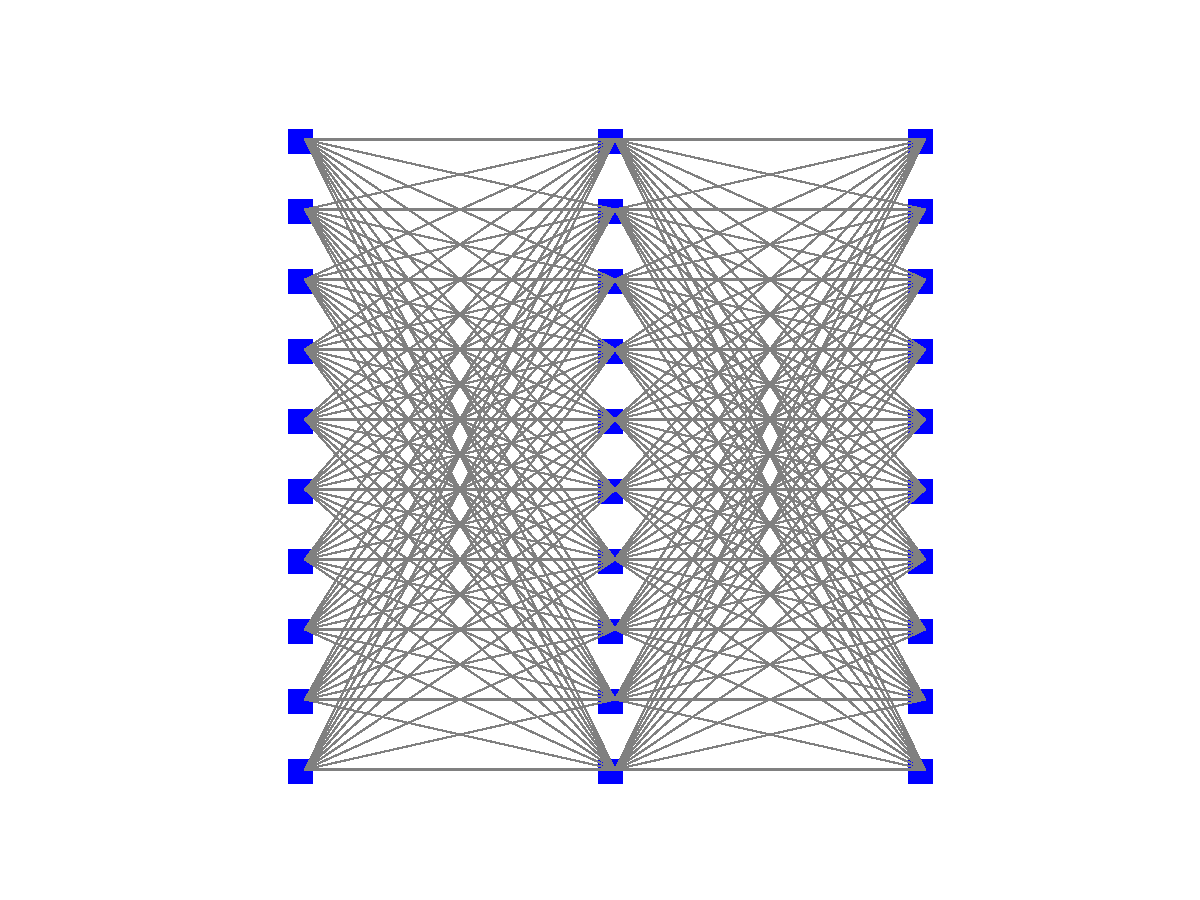
\includegraphics[width=1\textwidth]{images/img9}
%		\caption{پارامتر‌های مدارمعادل \lr{STT-RAM}}
%		\label{پارامترهای مدارمعادل STT-RAM}
%	\end{figure}
%	
%	در کدهای نوشته شده نیز دقیقا همین معادلات طراحی و پیاده سازی شده است که به دلیل طولانی بودن کدها، آن ها را در گزارش نیاوردیم اما می‌توانید آنها را از مسیر \texttt{code/STT-RAM/} بررسی کنید.
%	
%	نتیجه شبیه‌سازی برای یک سیکل نوشتن به صورت زیر گزارش می‌شود:
%
%\begin{figure}[h]
%	\centering
%	\includegraphics[width=1\textwidth]{images/img8}
%	\caption{خروجی شبیه‌سازی}
%	\label{خروجی شبیه‌سازی}
%\end{figure}
%
%		
%		
%		
%		
%		
%	\question
%	\textbf{شبیه‌ساز \lr{NVSim} را در حالت \lr{RAM} تنظیم کرده و همه انواع حافظه‌ها را برای طراحی \lr{RAM} ارزیابی کرده و پس از انجام ارزیابی و بررسی تفاوت میزان توان، ناخیر، مساحت و ... بهترین مدل را انتخاب کرده و دلیل این انخاب را توضیح دهیدو}
%	
%	پس از نصب و بیلد شبیه‌ساز \texttt{NVSim} که توضیحات آن را مفصلا در تمرین سری اول دادیم\footnote{می‌توانید فایل ارائه را از \href{github.com/M-Sc-AUT/M.Sc-Computer-Architecture/tree/main/Memory Technologies/Presentation/02-Memory Technologies Simulators}{\textcolor{magenta}{اینجا}} دریافت کنید}
%	به سراغ تنظیم کردن فایل کانفیگ می‌رویم. فایل کانفیگ \texttt{NVSim} به‌نام \texttt{nvsim.cfg} است که اگر آن را باز کنیم مشابه با شکل «\textcolor{blue}{\ref{فایل کانفیگ NVSim}}» خواهد بود.
%	
%	
%	\begin{figure}[h]
%		\centering
%		\includegraphics[width=1\textwidth]{images/img1}
%		\caption{فایل کانفیگ NVSim}
%		\label{فایل کانفیگ NVSim}
%	\end{figure}
%	
%	در این قسمت می‌خواهیم حافظه های زیر را شبیه‌سازی کنیم:
%	\begin{latin}
%		\begin{enumerate}
%			\item DRAM
%			\item SRAM
%			\item STT-RAM
%			\item ReRAM
%			\item PCRAM\footnote{Phase change}
%			\item FeFET
%		\end{enumerate}
%	\end{latin}
%	
%	از این رو، پارامتر‌های مشترک میان همه شبیه‌سازی‌ها را به‌صورت زیر تنظیم‌می‌کنیم:
%	\begin{latin}
%		\begin{enumerate}
%			\item \texttt{-DesignTarget: RAM}
%			\item \texttt{-CacheAccessMode: Normal}
%			\item \texttt{-OptimizationTarget: ReadLatency}
%			\item \texttt{-OptimizationTarget: WriteLatency}
%			\item \texttt{-OptimizationTarget: Area}
%			\item \texttt{-EnablePruning: Yes}
%			\item \texttt{-ProcessNode: 32}
%			\item \texttt{-Capacity (KB): 128}
%			\item \texttt{-WordWidth (bit): 512}
%			\item \texttt{-DeviceRoadmap: HP}
%			\item \texttt{-LocalWireType: LocalAggressive}
%			\item \texttt{-LocalWireRepeaterType: RepeatedNone}
%			\item \texttt{-LocalWireUseLowSwing: No}
%			\item \texttt{-GlobalWireType: GlobalAggressive}
%			\item \texttt{-GlobalWireRepeaterType: RepeatedNone}
%			\item \texttt{-GlobalWireUseLowSwing: No}
%			\item \texttt{-Routing: H-tree}
%			\item \texttt{-InternalSensing: true}
%			\item \texttt{-Temperature (K): 350}
%			\item \texttt{-BufferDesignOptimization: balance}
%			\item \texttt{-ForceBank (Total AxB, Active CxD): 4x4, 1x4}
%			\item \texttt{-ForceMat (Total AxB, Active CxD): 2x2, 1x2}
%			\item \texttt{-ForceMuxSenseAmp: 2}
%			\item \texttt{-ForceMuxOutputLev1: 1}
%			\item \texttt{-ForceMuxOutputLev2: 1}
%		\end{enumerate}
%	\end{latin}
%	
%	تمام فایل‌های سلول های مدنظر، در مسیر \texttt{sample\_cells/} موجود است. فقط می‌بایست نام سلول را از فایل کانفیگ \texttt{nvsim.cfg} تغییر دهیم. سپس می‌توان فایل کانفیگ را با دستور زیر شبیه‌سازی کرد:
%	\begin{latin}
%		 \texttt{./nvsim nvsim.cfg} 
%	\end{latin}
%	
%	پس از انجام شبیه‌سازی برای تمام حالت‌های گفته شده، نتایج به صورت زیر خلاصه می‌شود:
%	
%	
%	\begin{latin}
%		\begin{center}
%			\resizebox{\columnwidth}{!}{%
%			\begin{tabular}{||c | c c c c c c c c||} 
%				\hline
%				&\thead{\textbf{Total}\\ \textbf{Area}} & \thead{\textbf{Read}\\ \textbf{Latency}} & \thead{\textbf{Write}\\ \textbf{Latency}} & \thead{\textbf{Read}\\ \textbf{BandWidth}} & \thead{\textbf{Write}\\ \textbf{BandWidth}} & \thead{\textbf{Read}\\ \textbf{Dynamic}\\ \textbf{Energy}} & \thead{\textbf{Write}\\ \textbf{Dynamic}\\ \textbf{Energy}} & \thead{\textbf{Leakage}\\ \textbf{Power}} \\ [0.5ex] 
%				\hline\hline
%				\textbf{DRAM} & - & - & - & - & - & - & - & -\\ 
%				\hline
%				\textbf{SRAM} & \thead{185362.692\\$\mu m^2$} & \thead{\textbf{627.910}\\\textbf{$ps$}} & \thead{611.142\\$ps$} & \thead{225.114\\$\frac{GB}{s}$} & \thead{\textbf{125.293}\\\textbf{$\frac{GB}{s}$}} & \thead{67.322\\$pJ$} & \thead{64.013\\$pJ$} & \thead{204.144\\$mW$}\\
%				\hline
%				
%				\textbf{STT-RAM} & \thead{85540.685\\$\mu m^2$} & \thead{1.817\\$ns$} & \thead{10.729\\$ns$} & \thead{56.605\\$\frac{GB}{s}$} & \thead{6.016\\$\frac{GB}{s}$} & \thead{147.588\\$pJ$} & \thead{567.153\\$pJ$} & \thead{8.448\\$mW$}\\
%				\hline
%				
%				\textbf{ReRAM} & \thead{47398.933\\$\mu m^2$} & \thead{1.508\\$ns$} & \thead{20.474\\$ns$} & \thead{45.200\\$\frac{GB}{s}$} & \thead{3.139\\$\frac{GB}{s}$} & \thead{104.113\\$pJ$} & \thead{378.342\\$pJ$} & \thead{33.457\\$mW$}\\
%				\hline
%				
%				\textbf{PCRAM} & \thead{\textbf{22529.945}\\\textbf{$\mu m^2$}} & \thead{483.826\\$ps$} & \thead{\textbf{Reset latency} \\\textbf{40.448}\\\textbf{$ps$}} & \thead{239.386\\$\frac{GB}{s}$} & \thead{425.603\\$\frac{MB}{s}$} & \thead{28.223\\$pJ$} & \thead{Rest\\51.880\\$nJ$} & \thead{7.705\\$mW$}\\
%				\hline
%				
%				\textbf{FeFET} & \thead{23014.816\\$\mu m^2$} & \thead{346.615\\$ps$} & \thead{Reset\\1.340\\$\mu s$} & \thead{\textbf{265.731}\\\textbf{$\frac{GB}{s}$}} & \thead{47.756\\$\frac{MB}{s}$} & \thead{\textbf{23.481}\\\textbf{$pJ$}} & \thead{\textbf{Reset}\\\textbf{51.808}\\\textbf{$pJ$}} & \thead{\textbf{7.598}\\\textbf{$mW$}}\\ [1ex]
%				\hline
%			\end{tabular}
%		}
%		\end{center}
%	\end{latin}
%	
%	تمامی شبیه‌سازی‌ها برای یک سلول $4\times4$ انجام شده است. ظرفیت هر حافظه  $128 \text{KB}$ و عرض باس داده $64\text{B}$ درنظر گرفته شده است.
%	
%	طبق نتایج حاصل از شبیه‌سازی مشاهده می‌شود که کمترین مساحت مصرفی را \lr{PCRAM} دارد، همچنین کمترین تاخیر در خواندن متعلق به \lr{SRAM} است و کمترین تاخیر در نوشتن را \lr{PCRAM} دارد. بیشترین پهنای باند خواندن، کمترین انرژی خواندن و نوشتن، و کمترین توان مصرفی به \lr{FeFET} تعلق دارد، همچنین بیشترین پهنای‌باند در نوشتن را \lr{SRAM} دارد.
%	
%	نمی‌توان از میان این حافظه‌ها یکی را انتخاب کرد، چرا که انتخاب ما کاملا بستگی به اپلیکیشن دارد. ممکن است در یک اپلیکیشن صرفا مساحت مصرفی تراشه اهمیت زیادی داشته باشد و تاخیر در نوشتن چندان اهمیتی نداشته باشد. اما برای آنکه بتوانیم یکی را انتخاب کنیم، فرض می‌کنیم اپلیکیشنی داریم که:
%	
%	 \begin{itemize}
%	 	\item محدودیتی در مساحت مصرفی نداریم
%	 	\item فقط تاخیر خواندن برایمان اهمیت دارد
%	 	\item فقط پهنای باند خواندن مهم است
%	 	\item فقط انرژی مصرفی خواندن مهم است
%	 	\item و توان مصرفی هم برایمان مهم است
%	 \end{itemize}
%	 
%	 با این فرضیات دو گزینه را می‌توان انتخاب کرد. \lr{SRAM} و \lr{FeFET}. بر اساس کاربرد می‌بایست مصالحه\footnote{Tradeoff} ای بین این‌دو انجام دهیم و درنهایت یکی‌را انتخاب کنیم.
%	
%	خروجی شبیه‌سازی‌ها در مسیر زیر وجود دارد:
%	
%	\begin{latin}
%		\texttt{code/nvsim-merged/Results/}
%	\end{latin}
%	
%	
%	خروجی شبیه‌سازی برای \lr{DRAM} با خطای زیر مواجه می‌شود که متاسفانه نتوانستم علت خطا را پیدا و آن را رفع کنی.
%	\begin{latin}
%		\texttt{[ERROR] DRAM model is still under development} 
%	\end{latin}
%	
%	\begin{figure}[h]
%		\centering
%		\includegraphics[width=1\textwidth]{images/img2_DRAM}
%		\caption{خروجی شبیه‌سازی DRAM}
%		\label{خروجی شبیه‌سازی DRAM}
%	\end{figure}
	
 \end{questions}

\end{document}